\documentclass[10pt,
% a4paper,
%twocolumn,
fleqn,
%landscape, 
% papersize,
dvipdfmx,
uplatex
]{jsarticle}



\def\maru#1{\textcircled{\scriptsize#1}}%丸囲み番号

% \RequirePackage[2020/09/30]{platexrelease}

%太字設定
\usepackage[deluxe]{otf}

\usepackage{emathEy}

\usepackage[g]{esvect}

%定理環境
\usepackage{emathThm}
%\theoremstyle{boxed}
\theorembodyfont{\normalfont}
\newtheorem{Question}{問題}[subsection]
\newtheorem{Q}{}[subsection]
\newtheorem{question}[Question]{}
\newtheorem{quuestion}{}[subsection]

%セクション,大問番号のデザイン
\renewcommand{\labelenumi}{(\arabic{enumi})}
\renewcommand{\theenumii}{\alph{enumii})}
\renewcommand{\thesection}{第\arabic{section}章}

%用紙サイズの詳細設定
\usepackage{bxpapersize}
\papersizesetup{size={80mm,45mm}}
\usepackage[top=0.7zw,bottom=0truemm,left=3truemm,right=133truemm]{geometry}
\usepackage[dvipdfmx]{graphicx}

%余白など
\usepackage{setspace} % 行間
\setlength{\mathindent}{1zw}
\setlength\parindent{0pt}


%色カラーに関する設定
\usepackage{color}
\definecolor{shiro}{rgb}{0.95703125,0.87109375,0.7421875}
\definecolor{kin}{rgb}{0.95703125,0.87109375,0.7421875}
\definecolor{orange}{rgb}{1,0.7,0.2}
\definecolor{bradorange}{rgb}{1,0.5,0}
\color{kin}
% \pagecolor{hukamido}

\usepackage{at}%図の配置
% \usepackage{wallpaper}

\begin{document}




\at(0cm,0cm){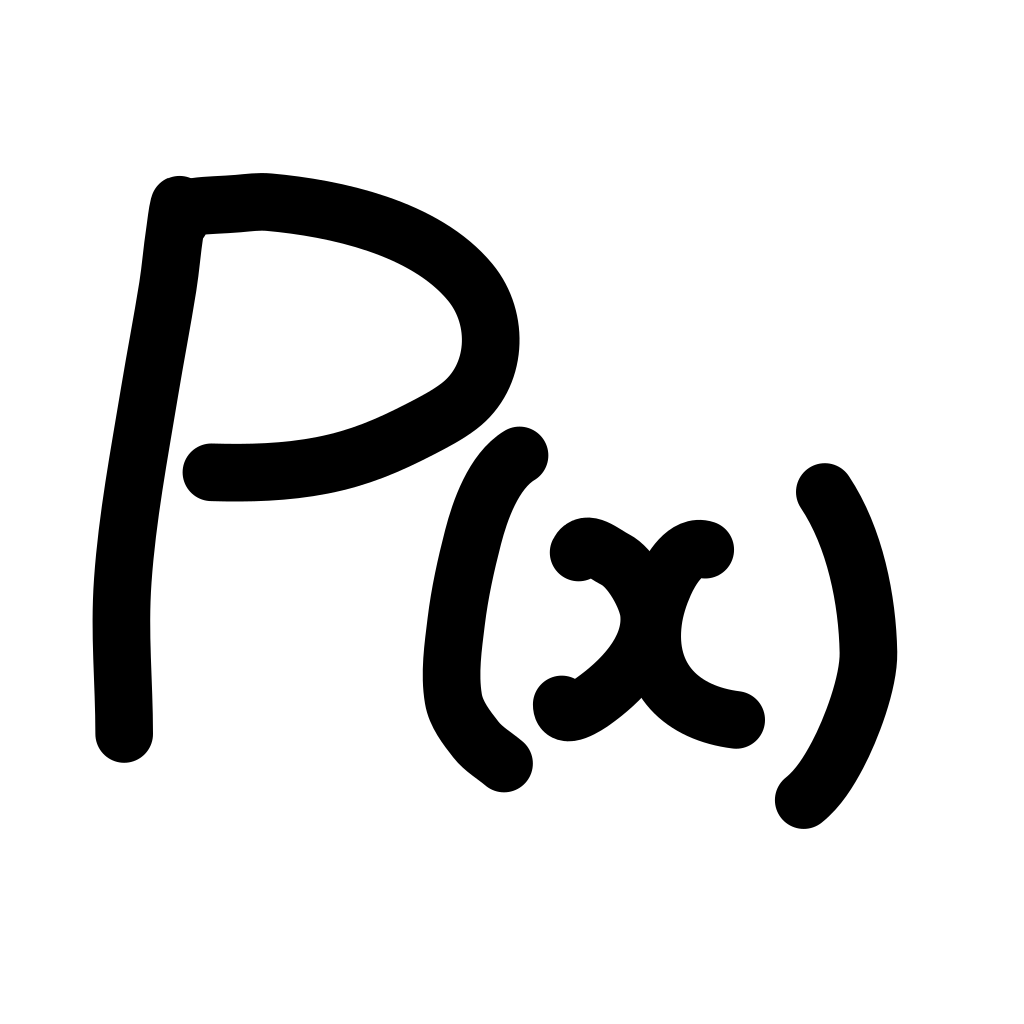
\includegraphics[width=8cm,bb=0 0 1920 1080]{./media_local/smart_background/複素数と方程式.jpeg}}
{\color{orange}\bf\boldmath\LARGE\underline{対称式の連立方程式}}\vspace{0.3zw}

\large 
\bf\boldmath 問.$x,\;y$の連立方程式


\Large
\vspace{0.1zw}
\hspace{0.5zw}$\left\{\begin{array}{l}\vspace{0.1zw}2x+2y+xy=3a-1,\vspace{-0.1zw}\\x+y+xy=a\end{array}\right.$
\vspace{0.1zw}

\large 
が$x,\;y$が実数である解をもつような実数$a$の範囲を求めよ.
\at(6.4cm,0.2cm){\small\color{bradorange}$\overset{\text{複素数と方程式}}{\text{典型}}$}


\newpage



\at(0cm,0cm){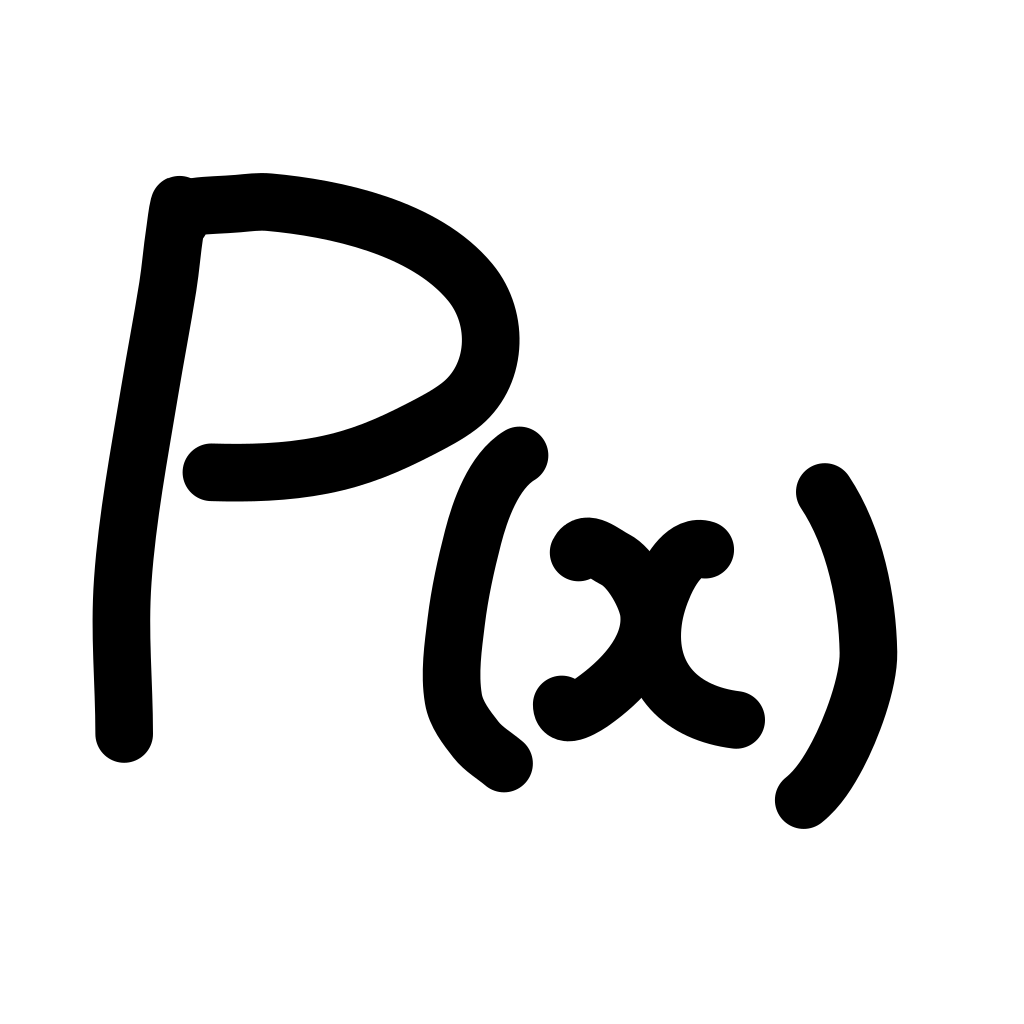
\includegraphics[width=8cm,bb=0 0 1920 1080]{./media_local/smart_background/複素数と方程式.jpeg}}
{\color{orange}\bf\boldmath\Large\underline{解の条件 〜解と係数の関係〜}}\vspace{0.3zw}

\large 
\bf\boldmath 問.方程式$2x^2+ax+6=0$の

\huge
$2$解のうち,\\
\hfill 一方が他方の$3$倍\vspace{0.3zw}

\large 
\hfill 
であるように実数$a$の値を定めよ.
\at(6.4cm,0.2cm){\small\color{bradorange}$\overset{\text{複素数と方程式}}{\text{典型}}$}


\newpage



\at(0cm,0cm){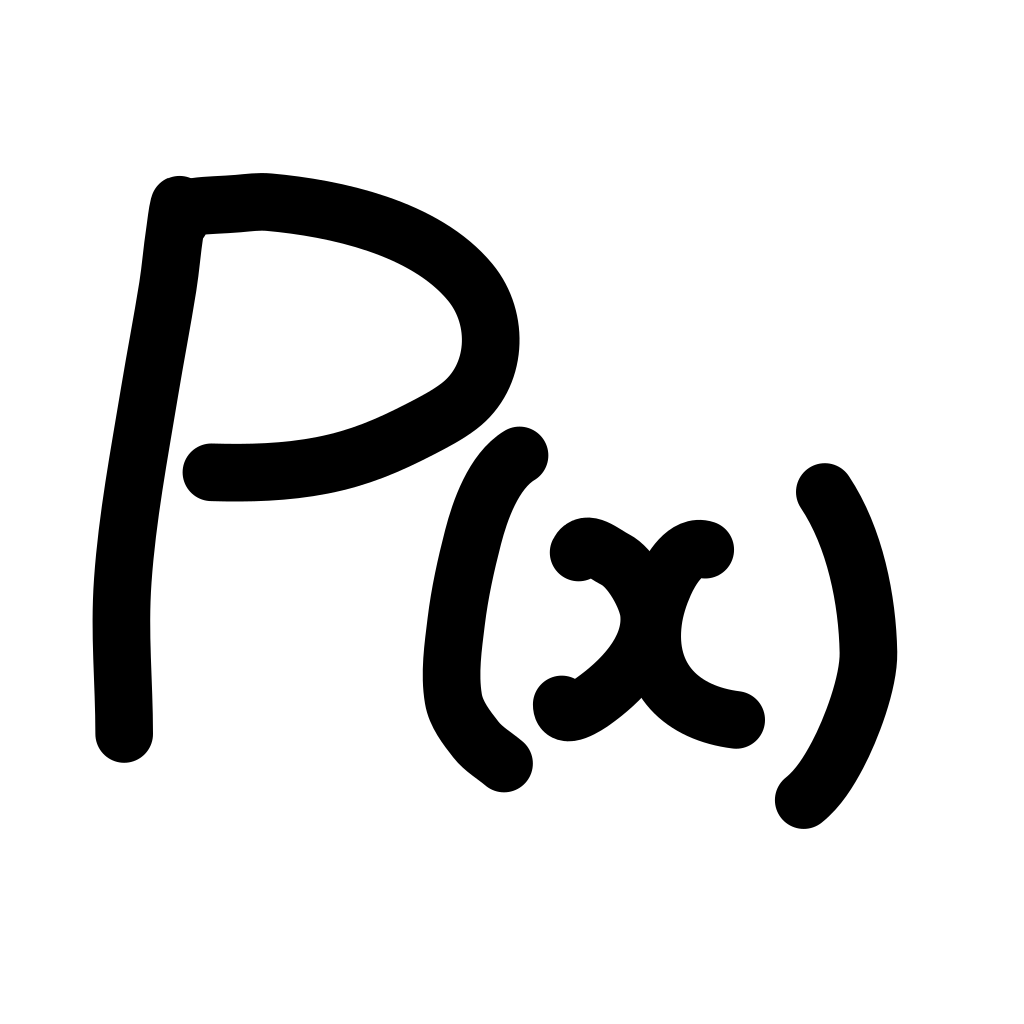
\includegraphics[width=8cm,bb=0 0 1920 1080]{./media_local/smart_background/複素数と方程式.jpeg}}
{\color{orange}\bf\boldmath\Large\underline{$2$解から$2$次方程式を作る}}\vspace{0.3zw}

\Large 
\bf\boldmath 問.方程式$3x^2-5x+1=0$の\\
$2$つの解を$\alpha ,\;\beta$とするとき,

\LARGE
\hspace{0.7zw}$\alpha ^3,\;\beta ^3$を$2$つの解にもつ

\Large
\hfill $2$次方程式を$1$つ作れ.
\at(6.4cm,0.2cm){\small\color{bradorange}$\overset{\text{複素数と方程式}}{\text{典型}}$}


\newpage



\at(0cm,0cm){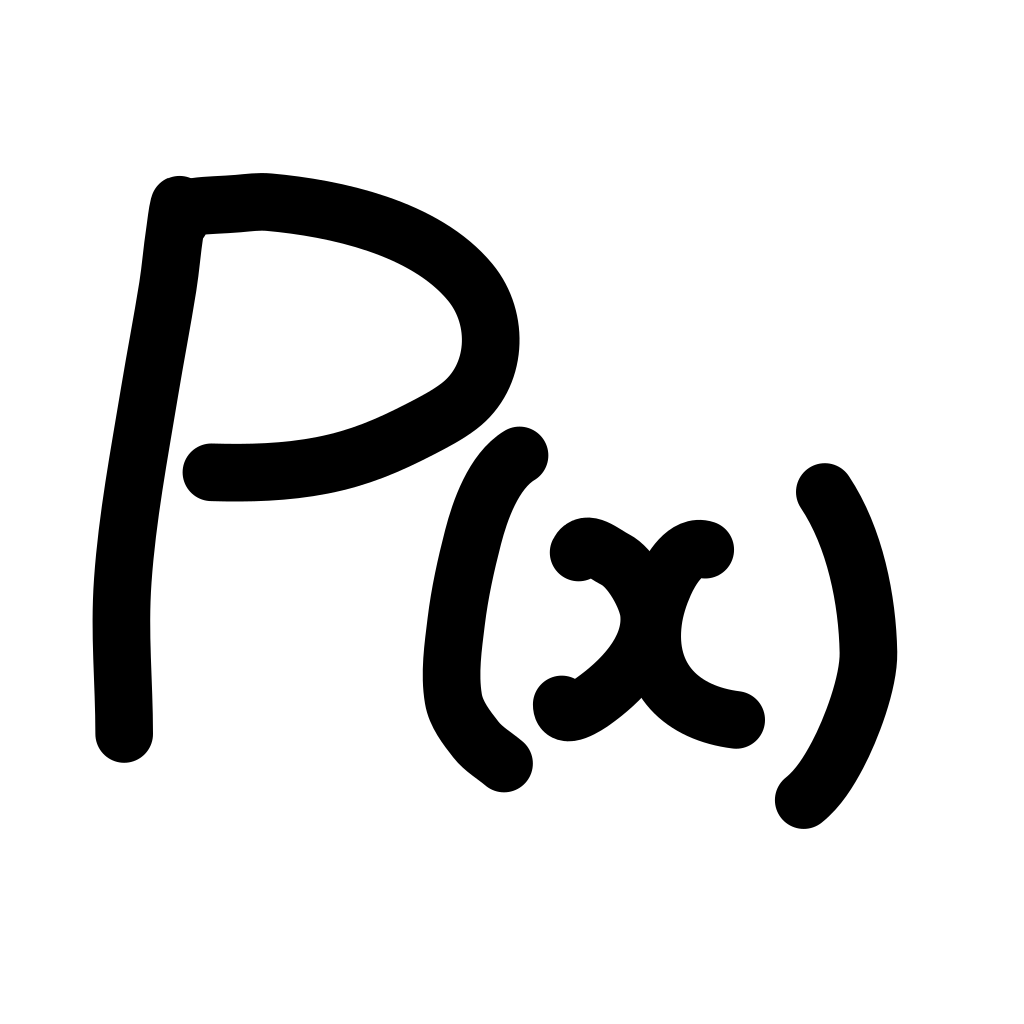
\includegraphics[width=8cm,bb=0 0 1920 1080]{./media_local/smart_background/複素数と方程式.jpeg}}
{\color{orange}\bf\boldmath\large\underline{$2$次方程式の$2$解$\alpha ,\;\beta$の対称式}}\vspace{0.3zw}

\Large 
\bf\boldmath 問.方程式$2x^2-3x+4=0$の\\
$2$つの解を$\alpha ,\;\beta$とおくとき,

\huge
\hspace{0.2zw}$\left(2-\alpha \right)\left(2-\beta \right)$
の値

\Large
\hfill を求めよ.
\at(6.4cm,0.2cm){\small\color{bradorange}$\overset{\text{複素数と方程式}}{\text{典型}}$}


\newpage



\at(0cm,0cm){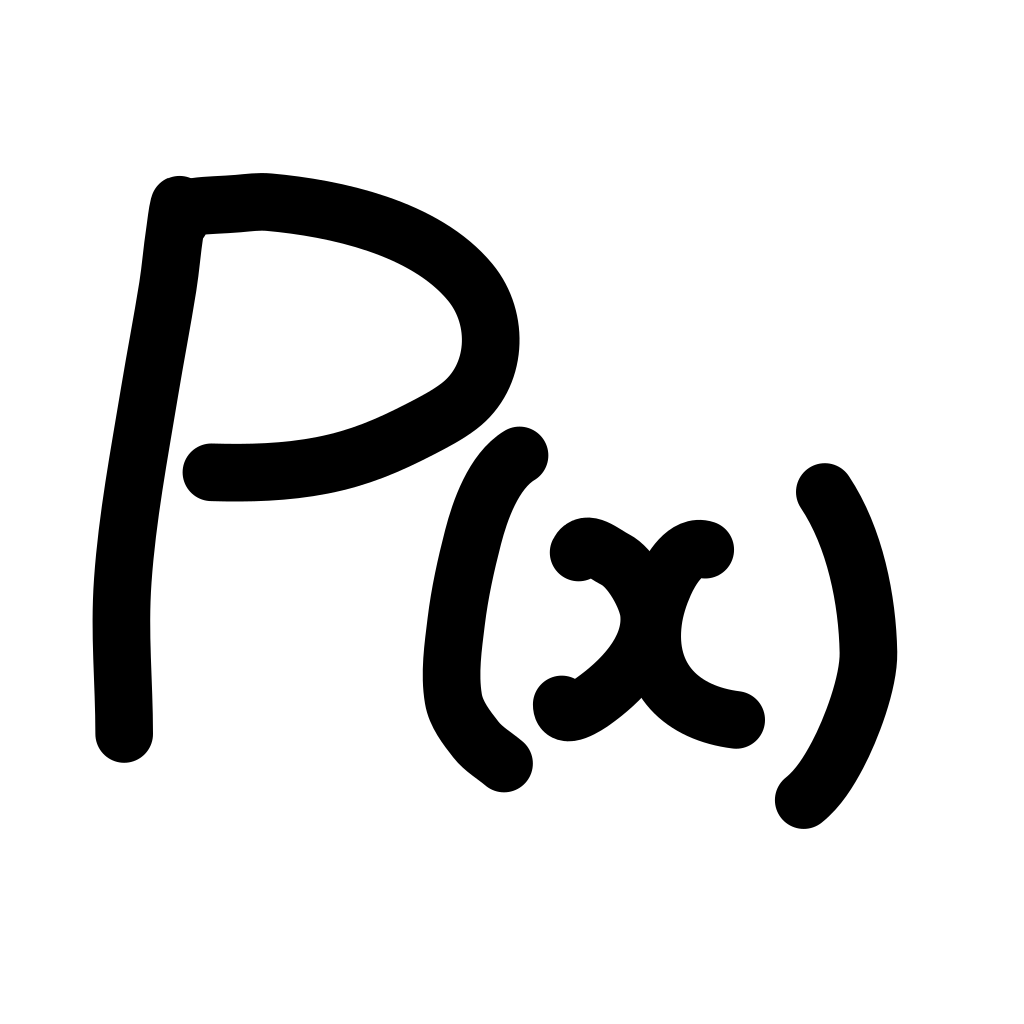
\includegraphics[width=8cm,bb=0 0 1920 1080]{./media_local/smart_background/複素数と方程式.jpeg}}
{\color{orange}\bf\boldmath\LARGE\underline{解と係数の関係の証明}}\vspace{0.3zw}

\large 
\bf\boldmath 問.$2$次方程式$ax^2+bx+c=0$において,次が成り立つことを示せ.

\Large
\vspace{0.2zw}
\hspace{0.2zw}$2$解が$x=\alpha ,\beta$である\vspace{0.2zw}

\large
\hfill $\iff$
\Large
$\alpha +\beta =-\bunsuu{b}{a},\;\alpha \beta =\bunsuu{c}{a}$
\at(6.4cm,0.2cm){\small\color{bradorange}$\overset{\text{複素数と方程式}}{\text{典型}}$}


\newpage



\at(0cm,0cm){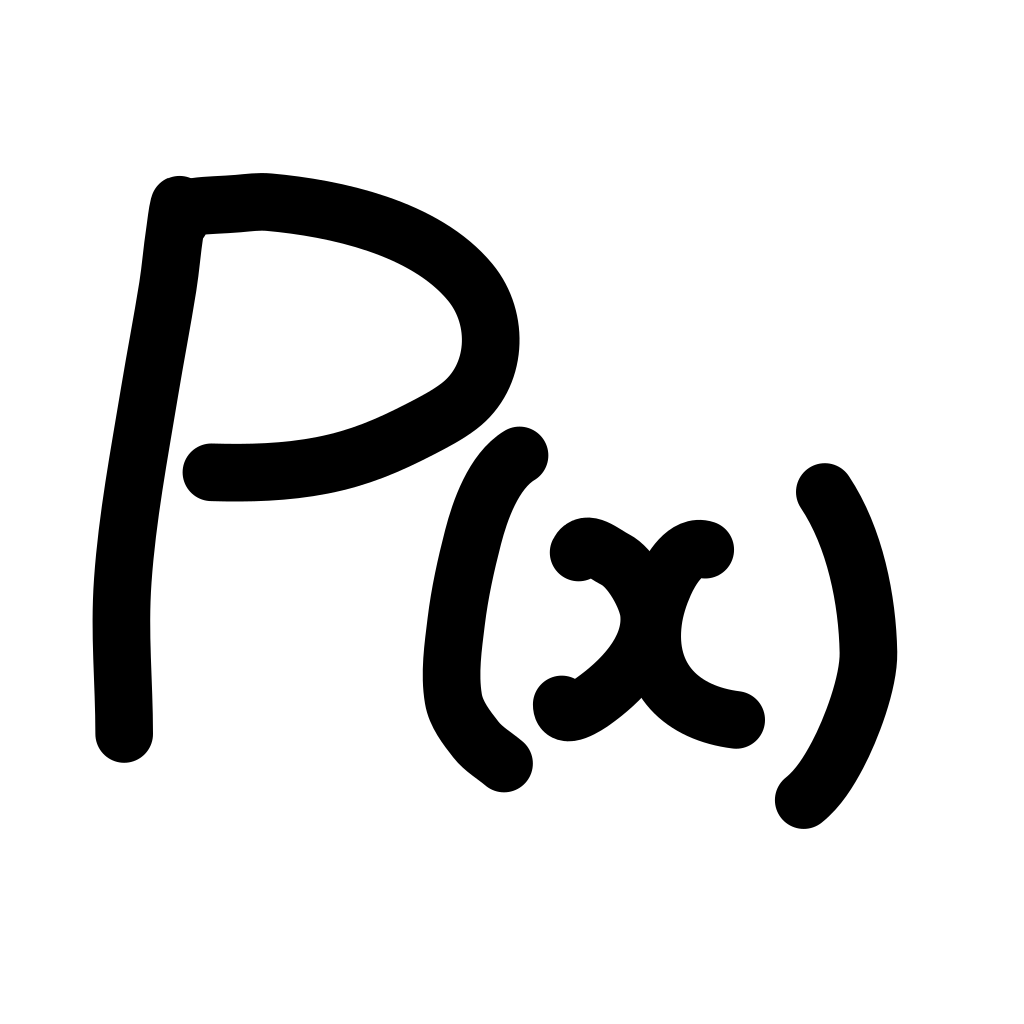
\includegraphics[width=8cm,bb=0 0 1920 1080]{./media_local/smart_background/複素数と方程式.jpeg}}
{\color{orange}\bf\boldmath\LARGE\underline{異なる$3$つの実数解}}\vspace{0.3zw}

\Large 
\bf\boldmath 問.$3$次方程式

\large 
\vspace{0.3zw}
\hspace{0.5zw}$x^3+\left(a-1\right)x^2-\left(a-4\right)x-4=0\vspace{0.3zw}$

\Large 
が異なる$3$つの実数解をもつような定数$a$の値の範囲を求めよ.
\at(6.4cm,0.2cm){\small\color{bradorange}$\overset{\text{複素数と方程式}}{\text{典型}}$}


\newpage



\at(0cm,0cm){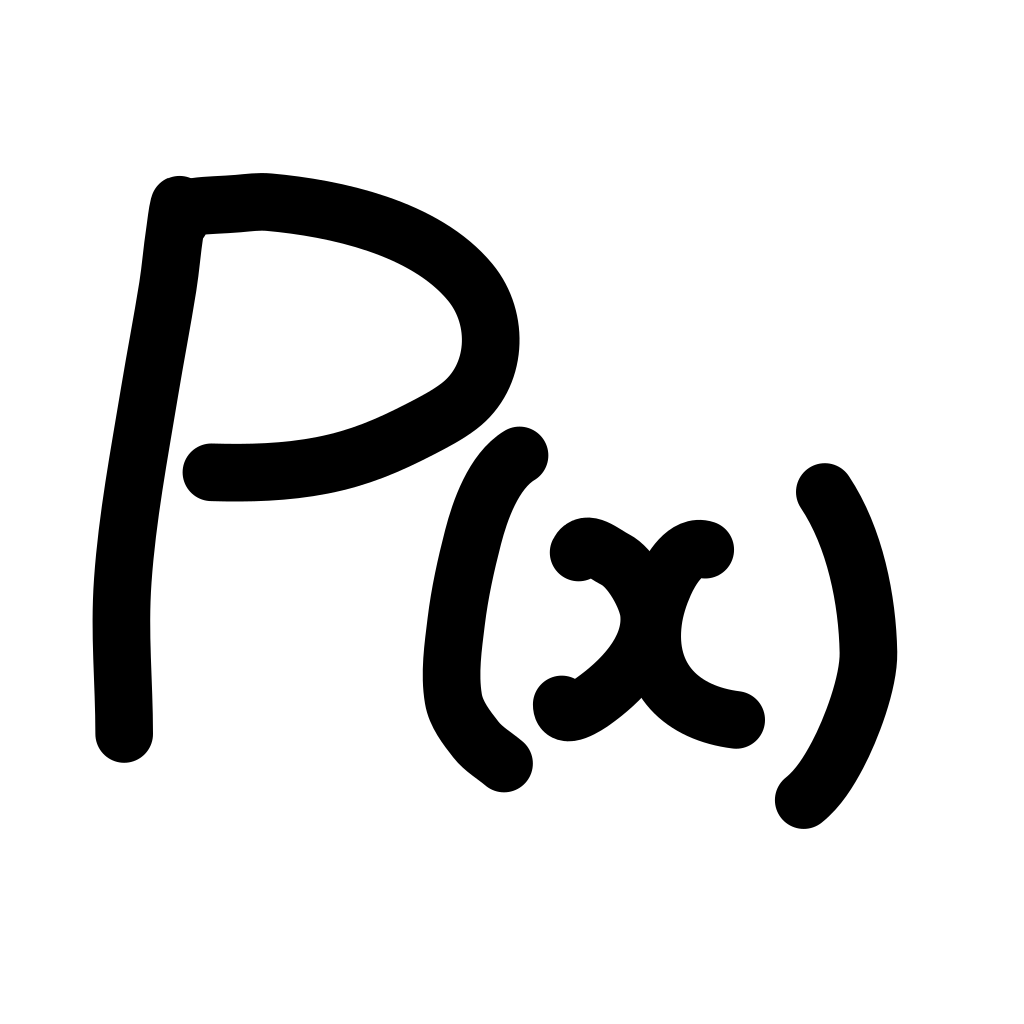
\includegraphics[width=8cm,bb=0 0 1920 1080]{./media_local/smart_background/複素数と方程式.jpeg}}
{\color{orange}\bf\boldmath\Large\underline{解の配置$〜$解と係数の関係$〜$}}\vspace{0.3zw}

\normalsize 
\bf\boldmath 問.$2$次方程式$x^2-2\left(m-2\right)x-m+{14}=0$が次のようなことなる$2$つの解を持つとき,定数$m$の値の範囲を求めよ.

\Large
(1)ともに正の解\hspace{0.2zw}(2)ともに負の解\vspace{0.2zw}

\normalsize
\hspace{0.2zw}(3)符号が異なる解\hspace{1.5zw}(4)ともに$1$より大きい\\

\at(6.4cm,0.2cm){\small\color{bradorange}$\overset{\text{複素数と方程式}}{\text{典型}}$}


\newpage



\at(0cm,0cm){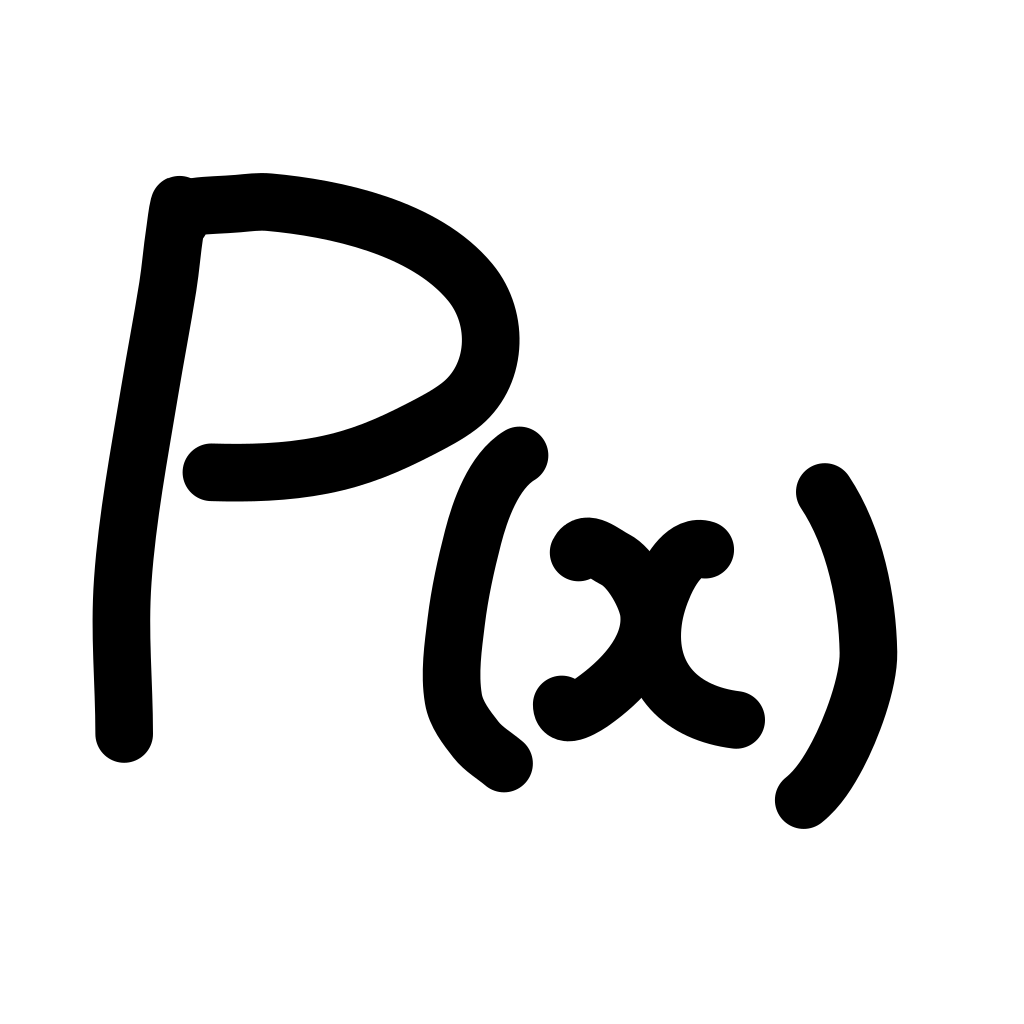
\includegraphics[width=8cm,bb=0 0 1920 1080]{./media_local/smart_background/複素数と方程式.jpeg}}
{\color{orange}\bf\boldmath\Large\underline{$2$重解をもつ$3$次方程式}}\vspace{0.1zw}

\LARGE 
\bf\boldmath 問.$3$次方程式

\hspace{0.2zw}$x^3+\left(a-4\right)x-2a=0$

が$2$重解をもつとき,

\vspace{-0.2zw}
\hfill 実数$a$の値を求めよ.
\at(6.4cm,0.2cm){\small\color{bradorange}$\overset{\text{複素数と方程式}}{\text{典型}}$}


\end{document}

